
\documentclass[10pt,landscape]{article}
\usepackage{multicol}
\usepackage{calc}
\usepackage{ifthen}
\usepackage{graphicx}
\usepackage[landscape]{geometry}
\usepackage{hyperref}

% To make this come out properly in landscape mode, do one of the following
% 1.
%  pdflatex latexsheet.tex
%
% 2.
%  latex latexsheet.tex
%  dvips -P pdf  -t landscape latexsheet.dvi
%  ps2pdf latexsheet.ps


% If you're reading this, be prepared for confusion.  Making this was
% a learning experience for me, and it shows.  Much of the placement
% was hacked in; if you make it better, let me know...


% 2008-04
% Changed page margin code to use the geometry package. Also added code for
% conditional page margins, depending on paper size. Thanks to Uwe Ziegenhagen
% for the suggestions.

% 2006-08
% Made changes based on suggestions from Gene Cooperman. <gene at ccs.neu.edu>


% To Do
% \listoffigures \listoftables
% \setcounter{secnumdepth}{0}


% This sets page margins to .5 inch if using letter paper, and to 1cm
% if using A4 paper. (This probably isn't strictly necessary.)
% If using another size paper, use default 1cm margins.
\ifthenelse{\lengthtest { \paperwidth = 11in}}
	{ \geometry{top=.5in,left=.5in,right=.5in,bottom=.5in} }
	{\ifthenelse{ \lengthtest{ \paperwidth = 297mm}}
		{\geometry{top=1cm,left=1cm,right=1cm,bottom=1cm} }
		{\geometry{top=1cm,left=1cm,right=1cm,bottom=1cm} }
	}

% Turn off header and footer
\pagestyle{empty}
 

% Redefine section commands to use less space
\makeatletter
\renewcommand{\section}{\@startsection{section}{1}{0mm}%
                                {-1ex plus -.5ex minus -.2ex}%
                                {0.5ex plus .2ex}%x
                                {\normalfont\large\bfseries}}
\renewcommand{\subsection}{\@startsection{subsection}{2}{0mm}%
                                {-1explus -.5ex minus -.2ex}%
                                {0.5ex plus .2ex}%
                                {\normalfont\normalsize\bfseries}}
\renewcommand{\subsubsection}{\@startsection{subsubsection}{3}{0mm}%
                                {-1ex plus -.5ex minus -.2ex}%
                                {1ex plus .2ex}%
                                {\normalfont\small\bfseries}}
\makeatother

% Define BibTeX command
\def\BibTeX{{\rm B\kern-.05em{\sc i\kern-.025em b}\kern-.08em
    T\kern-.1667em\lower.7ex\hbox{E}\kern-.125emX}}

% Don't print section numbers
\setcounter{secnumdepth}{0}


\setlength{\parindent}{0pt}
\setlength{\parskip}{0pt plus 0.5ex}


% -----------------------------------------------------------------------

\begin{document}

\raggedright
\footnotesize
\begin{multicols*}{4}


% multicol parameters
% These lengths are set only within the two main columns
%\setlength{\columnseprule}{0.25pt}
\setlength{\premulticols}{1pt}
\setlength{\postmulticols}{1pt}
\setlength{\multicolsep}{1pt}
\setlength{\columnsep}{2pt}

\section{1-2}
\textbf{Confidentiality} Only access to those wanted via i.e., access control\\
\textbf{Integrity} keep info correct, i.e., hash/MAC\\
\textbf{Availability} info available, i.e., make copies/distribute\\
\textbf{Authenticity/Integrity of origin} prevent fake info, i.e., keyed hash == MAC/ sign\\
\textbf{Non repudiation} prevent denial of statement, add signature\\
\textbf{Security lifecycle} Risk assessment$\rightarrow$ establish policy$\rightarrow$ implement$\rightarrow$operate maintain\\
\textbf{Commodity threats} targets everyone\\
\textbf{Rootkit} hide malware\\
\textbf{LDAP inject} (\&(name=admin)(\&))(pwd=...))\\
\textbf{Inject protection} inspect data twice (input validate, encode when use)\\
\textbf{Broken access control} ex. direct object ref\\

\section{3 - Crypto}
\textbf{Confidentiality - Integrity - Authentification - Non repudiation}\\
\textbf{Stream cipher} Malleable (flip bit), should use IV\\
\textbf{ECB} Encrypt each block separately$\rightarrow$still visible\\
\textbf{CBC} Chaining. Needs padding. Flip$\rightarrow$next block garbaged, next block flipped\\
\textbf{$2^{nd}$ pre-image} no collision for specific hash\\
\textbf{MAC} sym key. Auth \& integrity\\
\textbf{AEAD} best practice. Associated Data\\
\textbf{Dig. Sign.} encrypt hash msg\\
\textbf{ECC} smaller keys\\
\textbf{TLS} Server has cert. Sign client info (RSA) $\rightarrow$ sym. key (DH) and HMAC (SHA)\\
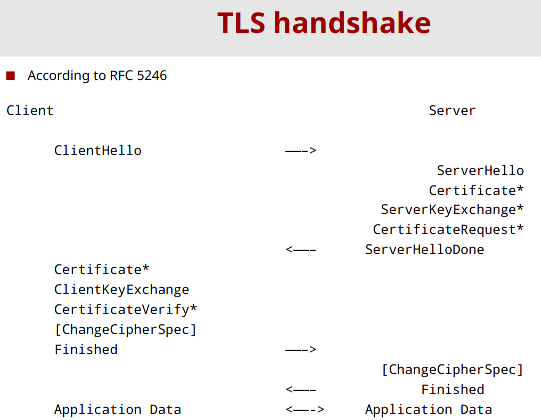
\includegraphics[width=\columnwidth]{tls.png}
\textbf{SNI} server name unencrypted\\
\textbf{HSTS} Remember HTTPS. Option to preload.\\
\textbf{Cert Pinning} Client knowns which CA can sign.\\

\section{4 DB security} 
\textbf{DB access \& encrypt} Hardware - OS - Database - Network - Application\\
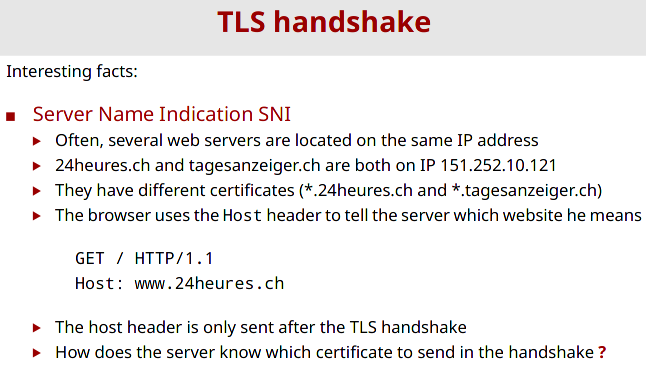
\includegraphics[width=\columnwidth]{tls2.png}
\textbf{DAC} discret. acc. control.  grant privilege on views/tables.\\
\textbf{Role based AC} grant role to users
\textbf{Rainbow} t memory look up, $\frac{1}{2}t^2$ hash op. m~x~t table\\
\textbf{PBKFD2} apply iterations standard\\
\textbf{Memory hard} Scrypt or Argon2\\
\textbf{DB encrypt} also encrypt in app but reduce utility.\\
\textbf{PAKE} pass. agreeed key exch.

\section{5 Access control}
\subsection{Access control}
\textbf{Least privilege}\\
\textbf{Role-based AC} simplify permissions by grouping users in roles, i.e., OS groups
\textbf{Adv.} easy idea, management, tell which perm. a user has.
\textbf{Disadv.} role granularity, role assignment\\
\textbf{Discreationary Access control} Object owen define access 
\textbf{Adv} easy, flexible \textbf{Disadv} owners judgement, risk of write unprotected copy.\\
\textbf{Access control list} each obj. know who can access
\textbf{Capabilities} each user know which object he can access (key).\\
\textbf{Linux ACL} \texttt{setuid/setgid} run as owner, i.e., \texttt{ping}\\
\textbf{Windows} ACL has delete, cap. $\rightarrow$ privileges\\
\textbf{Mandatory access control} Multilevel, subject can only access same or higher level, can be used with RBAC/DAC 
\textbf{Adv} address limit of DAC, scale
\textbf{DisAdv} can be too restrictive, not flexible\\
\textbf{MAC + Confid.} no write down $\rightarrow$ no trojan\\
\textbf{MAC + Integ.} no write up\\
\textbf{MAC} Windows integrity levels, Linux SELinux/AppArmor called right after DAC
\subsection{Authentication}
\textbf{Something you own} Bingo card, OTP, Transaction Auth. Number, pkey in hw.\\
\textbf{OATH} OTP from see, counter or time based\\
\textbf{U2F} FIDO2, pubkey to server, send challenge \textbf{Adv.} server/client hack fine\\
\textbf{Biometrics registration} acquire, extract char., store char.
\textbf{Bio auth} acquire, compare, decide
\textbf{Disadv.} acquisition never exact$\rightarrow$ no hash, no change\\
\textbf{Challenge response} challenge with pass. hash, MITM risk if not HMAC, mutual i.e., WPA2\\
\textbf{Kerberos} based on sym. keys and tickets system, 3 step approach, MITM not possible due to session key, replay attack not possible due to freshness and server keeping list of past ones\\
\textbf{Kerb. ticker} ticker usually valid 8h, $c$ client identity, $a$ IP address, $v$ validity period, $K_{c,s}$ session key between client and server, $T_{c,s}=\texttt{ENC}_{K_s}(c,a,v,K_{c,s})$\\
\textbf{Authenticator} $ENC_{K_{c,s}}(c,t)$\\
\textbf{Authentification} Password hash as $K_c$, 1. client sent c, tgs for ticket to ticket granting system, authentification server responds with ticket granting ticker: $T_{c,tgs}$ and session key: $ENC_{K_c}(K_{c,tgs})$\\
\textbf{Authorization} client create authenticator with $K_{c,tgs}$, send $T_{c,tgs}$ and $A_{c,tgs}$ to the TGS, TGS checks A and send back $T_{c,s}$ and an encrypted session key $ENC\_{K_{c,tgs}}(K_{c,s})$, client knows $K_{c,tgs}$ and can decrypt session key\\
\textbf{Access} client create $K_{c,s}$, sends $T_{c,s}$ and $A_{c,s}$, server verifies and then allows service\\
\textbf{Ticket validation} decrypt, validate IP and period, use session key to: decrypt authentificator, verify it contains same id c as ticket, then verify authenticator is fresh + that authenticator not used in last 5min\\
\textbf{Kerb. attack} Request ticket for user c, bruteforce session key $K_{c,tgs}$ with pass. hashes, countered by pre-auth: user send authenticator to TGT, bruteforcing possible but you can observe when user login\\
\textbf{Preauth} client create authentificator $K_c(pwd hash, sals, iteration)$, client ask for ticket at TGS, sends c, tgs, and $A_c$, AS response with $T_{c,tgs}$ and $ENC_{K_c}(K_{c,tgs})$\\
\textbf{Microsoft} $K_c$ not password hash, many iterations\\
\textbf{kerb sec.} relies on sym. keys: pass. hash, sym. keys to encrypt ticket\\
\subsection{Delegated auth}
\textbf{Oauth2} roles: client, resource server, authorization server, user --- client and auth have shared secret, client exchange authentification code for access token --- most apps store no pass. but store oauth token\\
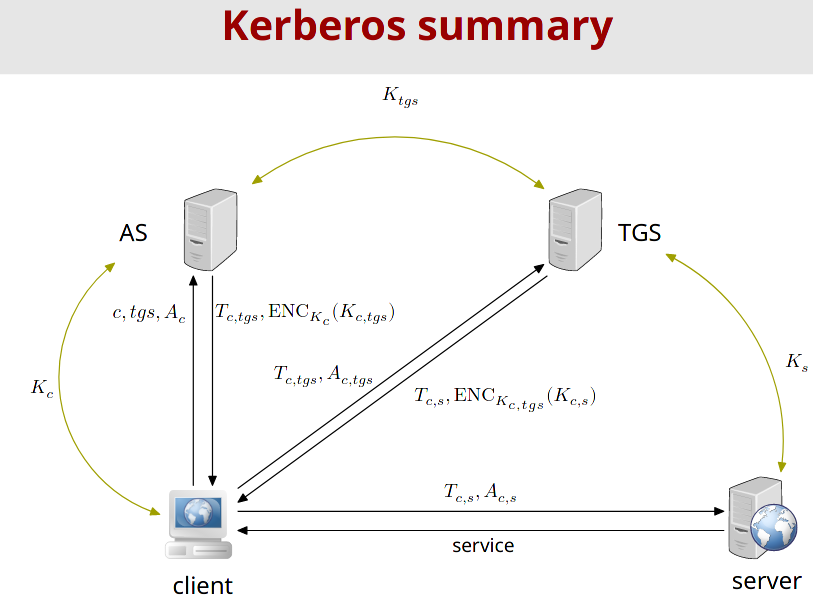
\includegraphics[width=\columnwidth]{kerb.png}\\
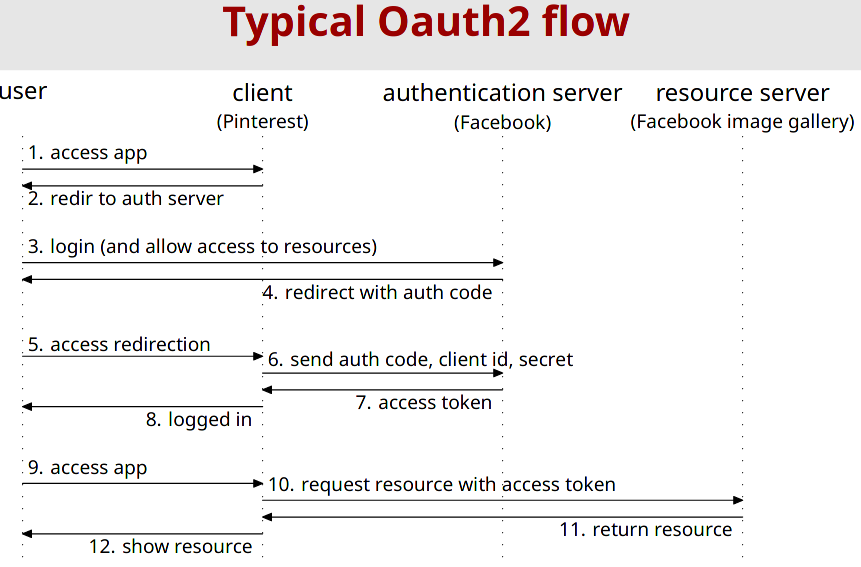
\includegraphics[width=\columnwidth]{oauth2.png}\\

\section{6 Netsec}
\textbf{Network segmenation} via ACL, rings vs zone\\
\textbf{DMZ} single FW, or dual www - FW - DMZ -FW - LAN\\
\textbf{Zero trust} 8body is evil, easy to implement, cost to run\\
\textbf{Default deny}
\textbf{Signature based IDS} i.e., Snort, WAF style in front of FW\\
\textbf{Privilege esc.} replace system program with malicious one\\
\textbf{Backup} Full - incremental - differential, 3 copies - 2 media - 1 add. site.\\
\textbf{Disaster reocvery plan} DRP\\

\section{7 Trusted Computing}
\textbf{TPM} chip + memory (non-volatile, Platform config. reg.)\\
\textbf{Attestation} prove certain state (hw, OS, codwidelye). i.e., secure boot, signal\\
\textbf{Att. Id. Key} pkey in TPM, pubkey cert by Authority\\
\textbf{Sealing} store priv. info. bound to specific state, Only decrypt if same state, i.e., bitlocker (Vol. Master Key sealed)\\
\textbf{Isolation} mechanism limit who has access$\rightarrow$tamper resistance/evident/responsive\\
\textbf{HSM} tamper resistant, mostly crypo, FIPS level certified, API=PKCS\#11\\
\textbf{iOS backup} HSM pubKey in device, send passcode and get enc key, to decrypt passcode check, counter\\
\textbf{Side channel fix} Hiding (lower signal), Masking (deal with masked values), Prevent leakage

\section{8 9 Privacy}
\textbf{function creep} divert from original goal\\
\subsection{Privacy by desing and default}
\textbf{Proactive + Preventive} -- \textbf{Per Default} -- \textbf{Embedded into design} -- \textbf{Positive Sum} -- \textbf{Full lifecycle protection} -- \textbf{Visibility, transparency, open} -- \textbf{User centric}\\
\subsection{PETs paradigms}
\textbf{Confidentiality} minimized data disclosure, distribute trust, open-source\\
\textbf{Control} User participation, transparency + accountability, organized compliance (FIPP/GDPR)\\
\textbf{Practice} Improve user agency, aid decision making, collective practice\\
\subsection{Pets Adversary class}
\textbf{Social} defined by users, help decision + detect impact
\textbf{Lim.} trust service provider\\
\textbf{Institutional} defined by law, informed consent + purposed limit. + data minimization + access right
\textbf{Lim.} reliance on punishment, focus on misuse not collection, if compliant$\rightarrow$ok
\textbf{Anti-Surveillance} evade global adversary, minimize need to trust/reveal, E2E + obfusc. + PIR + TOR + Adv. Crypo (MultiParty..)
\textbf{Lim.} general purpose priv. is hard, usability for dev. and user, no incentives\\
\subsection{Tech PET}
\textbf{Anonymous Comm.} special routing\\
\textbf{Anonymous Cred.} Prove given appropriate cred.,prop: identity provider/verifier, unforgeability / selective disclosure / issuer unlinkability / verifier unlinkability\\
\textbf{Blind sign.} content of msg is blinded before signed. i.e., anonym. voting\\
\textbf{Sec. Multi party comm.} compute without exposing data\\
\textbf{Garbled circuits} B create circuit, A add input. Nobody learn\\
\textbf{Deterministic enc.} Good for search data\\
\textbf{Homomorphic enc.} Computation on cipher, i.e, Pallier\\
\textbf{Private set Intersection}\textbf{Private info retrieval}\\
\textbf{Oblivious Ram} PIR with R/W, hide which data is used\\
\textbf{Privacy properties} Confidentiality, Pseudonimity, Anonymity, Unlinkability, Unobservability, Plausible deniability\\
\textbf{Measuring priv.} Correctness, uncertainty, accuracy, differential priv. based
\textbf{k-anonimity} cannot distinguished from at least k-1 other persons\\
\textbf{Homogeinity attack} lack diversity\\
\textbf{l-diversity} every equiv. class need l well represented value\\
\textbf{t-closeness} dist. between distri. of sensitive attribute in the class and in the whole table is $\leq$ threshold t\\
\textbf{Simulatable auditing}
\textbf{Subsample} statistics on subset\\
\textbf{Input perturbation} Data modified before response\\
\textbf{Randomized response} randomness avg. out so still useful\\
\textbf{Differential priv.} Quantify leakage, small change in DB do no change distri., minimize increased risk when joining DB\\
$P[A(D)\in S] \leq e^\epsilon \cdot P[A(D_{-r})\in S]$\\
higher sensitivity ye higher distortion, (privacy guarantee $\rightarrow$ higher distortion (Laplace),
lower $\epsilon\rightarrow$ more privacy\\
\textbf{epsilon} add for multiple output, depends on sensitivity, 
\textbf{DP tools} add noise to DB, to algo, output\\
\textbf{ZK proof} zk-STARK for DNA, prop: completeness soundness zk,

\section{10 ML}
\textbf{Adversary goals} Steal data info, Steal model, fool user\\
\textbf{Steal linear model} d+1 queries\\
\textbf{Membership inference} Was x in the dataset? works because of overfitting,\\
\textbf{MI 3 poss. assumptions} No samples of training data, no knowledge of the distri. of training data, no knowledge of the model param.\\
\textbf{Attribute inference} Given answer, infer if a training sample had an attribute\\
\textbf{Privacy problems} ML needs data to learn, obtain value via giving sample (predict on noise$\rightarrow$reduced utility), the output reveal info (MI, attribute inference), ML good at inference\\ 
\textbf{Adverserial ex.} Input to make ML fail, transferable between model\\
\textbf{Adverserial training} train against adv. ex.\\
\textbf{Certified defense} No adv. example exist up to certain perturbation\\
\textbf{Detect suspicious queries} look for deviation in successive queries\\
\textbf{Base rate} True positive * Reality / predictivness, hard to get good results on weak signals $P[attack|alarm]=\frac{P[alarm|attack]P[attack]}{P[alarm]}$\\
\textbf{Stat. bias} diff. between estimator exp. value and true value\\
\textbf{Group fairness} outcome should not differ between demographic groups\\
\textbf{Individual fairness} Should not differ between individuals\\
\textbf{Federated learning} Learn across datasets, build weights, each client compute updated weights, update model with weighted avg. of clients
\textbf{Lim.} need revel of model$\rightarrow$homomorphic enc./multiparty comm./Diff. priv.\\
\textbf{Privacy perseving distributed ML} Use multiparty homomorphic enc. which perform comp. without seeing the data\\
\textbf{}Combining decentralized data sets to train a ML model while protecting privacy is doable: adding noise to partial aggregates, sending partial aggregates to a trusted execution environment, By a combination of homomorphic encryption and secure multiparty computation\\

\section{12 Blockchain}
\textbf{Proof of personhood} Each human one vote / socialism\\
\textbf{Public} Anyone can write \textbf{Open} everyone can read\\
\textbf{Public + closed} i.e., voting\\
\textbf{Money: bearer instrument} Physical holder or holder of secret, easy transfer, anonymous can loose\\
\textbf{Registered instrument} Centralized record of ownership, can't lost it, not anonymous, transfer hard\\
\textbf{Forgery prevention} Scare resource + signature + legal recourse against forger\\
\textbf{Consensus properties} Termination: correct process will terminate, Integrity: if all correct propose x, then decide x, Agreement: everybody correct proposes same x\\
\textbf{Eclipse attack} Cut one node from network\\


\section{13 DNA}
\textbf{De-identification} Remove names\\
\textbf{Homer's attack} Learn if target is in the case group by correlating SNP\\
\textbf{GA4GH Beacon} check multiple DB for a specific question, attack possible by multiple query on lowest frequency allele\\
\textbf{Surname inference attack} Get lastname by looking at y chromosome, combine with age + sex for identification\\
\textbf{Multi site studies Health} multi party Homo. enc. (MHE) with honest but curious adversary and malicious but covert adversary.
\textbf{Distributed gradient descent} to create global model\\
\textbf{Single Nucleotide Polymorphism} At least one nucleotide different in $\geq$ 1\% pop, == alleles\\


\section{14 Evoting}
\textbf{Absence of provisional result} wait till end\\
\textbf{Individual verifiability} can check vote counted\\
\textbf{Universal verifiability} all votes correctly counted\\
\textbf{Control components} Gen. keys on 4 different setup, 1 trusted at least\\
\textbf{NKZIP} used to prove blinded vote same vote as encrypted and then mixed, correctly decrypted, know content of vote\\
\textbf{Elgamal} Provide multiplicative homomorphism, reencrypt with 1 to get anonymity, Prime order subgroup, $p=2q+1, g^{x mod q}mod p$, $\texttt{Enc}_{pk}(m,r)=(m\cdot pk^r, g^r), \texttt{ Dec}_{sk}(a,b)=a/b^{sk}=m$\\
\textbf{Key shares} decryption without knowing full key, enc(vote) with pubkey, each cc decrypt, sum pkeys, multiply pubkeys, enc. with pubkey, dec. with $b^{sk_j}$\\
\textbf{ZKP} $y=g^x$ pretend know x, publish y, commit w, publish $t=g^w$, challenge with c, publish s=cx+w, verify $g^s=ty^c$\\
\textbf{NIZKP} add text so that NIKZP is sign. for this card, two commitment on diff. g, hash of y*t
\textbf{vote} enc. vote v with elgamal $(v*pk^r, g^r)$, NIKZP they know random r, add some text to NIKZP, so text is signed\\
\textbf{Mixnets} change representations without changing content + shuffling, each CC mix, elgamal multiply enc(1) +NIZKP to prove didnt change content of vote\\
\textbf{Bugs} commitment, NIZKP where b can make gibberish while valid proof
$\Delta $
\end{multicols*}
\end{document}


\pagestyle{empty}